\documentclass{../industrial-development}
\graphicspath{{2-software-roles/}}

\title{Роли сотрудников в бизнес-процессах компании по разработке программного обеспечения.}
\author{Завойкин Алексей, ИТ-21 МО}
\date{}

\begin{document}

\begin{frame}
  \titlepage
\end{frame}

\begin{frame}{План лекции}
  \tableofcontents
\end{frame}

\section{Менеджер продукта }

\begin{frame} \frametitle{Менеджер продукта }
  
\end{frame}

\lecturenotes

Определение менеджера продукта часто напрямую зависит от определения менеджмента как такового. Менеджмент проекта – это совокупность знаний, навыков, инструментов и техник прилагаемых к проектным задачам с целью привести продукт к целям, поставленным заказчиком. Проектный менеджмент осуществляется через процессы инициирования, планирования, исполнения, наблюдения, контролирования и завершения. Проектный менеджер – человек, ответственный за выполнение всего вышеперечисленного. 
  ~\cite{Anatomy}
	
\begin{frame} \frametitle{Менеджер продукта: задачи}
  \begin{itemize}
	\item Установление критериев успеха
	\item Связь с клиентом
	\item Отслеживание статуса проекта
	\item Продвижение разработки вперед и преодоление проблем 
	\end{itemize}
\end{frame}

\lecturenotes

На ранних стадиях проекта менеджеры зачастую работают с функциональным аналитиком. В этой связке менеджер отвечает за критерии успеха и связь с клиентом. 
Проектный менеджер отвечает за отслеживанием статуса проекта. В разработке ПО именно эти менеджеры ответственны за продвижение разработки вперед и преодоление проблем. 
  ~\cite{Anatomy}

\begin{frame} \frametitle{Менеджер продукта: необходимая подготовка}
  \begin{itemize}
	\item Навыки функционального аналитика
	\item Навыки слушателя
	\end{itemize}
\end{frame}

\lecturenotes

Проектные менеджеры должны быть готовы выполнять определенную работу с постоянством. Должны быть готовы отступить от деталей и оценить проблемы целиком, готовы применить издержки личностного и командного характера. 
С целью сохранения рабочего процесса они также должны быть хорошими слушателями, чтобы убедиться, что проблема понята. 
Само заполучение роли зачастую спонтанно: архитектор решений или глава разработки выдвигает предложения по разработке и улучшению работы проекта, а также свою кандидатуру. Зачастую к роли приходят через роль функционального аналитика. 
  ~\cite{Anatomy}

\begin{frame} \frametitle{Менеджер продукта: инструментарий}
  \begin{itemize}
	\item Microsoft Project
	\item Шаблоны
	\end{itemize}
\end{frame}

\lecturenotes

ПО проектного менеджера, такое как Microsoft Project или Microsoft Project Server, является важнейшим элементом инструментария. Оно помогает документировать зависимости, статус, что помогает отслеживать состояние проекта. 
Шаблоны – процесс менеджмента может стать крайне утомительным при переизбытки генерируемой документации. Инструменты, позволяющие убедиться в том, что процессы в разработке текут максимально эффективным способом, есть в инструментарии каждого менеджера. 
  ~\cite{Anatomy}

\begin{frame} \frametitle{Менеджер продукта: достоинства роли}
  \begin{itemize}
	\item Заметность работы
	\item Связь с начальством и другими проектными менеджерами
	\item Высокая степень влияния на продукт
	\end{itemize}
\end{frame}

\begin{frame} \frametitle{Менеджер продукта: недостатки роли}
  \begin{itemize}
	\item Недостаток времени
	\item Переработка
	\end{itemize}
\end{frame}

\lecturenotes

К позитивным элементам роли относят высокую заметность работника (связь с начальством и другими проектными менеджерами), степень влияния на продукт и удовлетворенность от вовлеченности в результаты работы. 
К негативным элементам – недостаток времени и переработку. 
  ~\cite{Anatomy}

\begin{frame} \frametitle{Менеджер продукта: связь с другими ролями}
  \begin{itemize}
	\item Функциональный аналитик
	\item Специалист по контролю качества
	\end{itemize}
\end{frame}
\lecturenotes
Карьерный рост продукт-менеджера возможен в двух направлениях:

Вертикальном стремлении к более высокой позиции — групп-продукт-менеджер, начальник отдела маркетинга, директор по маркетингу;
Горизонтальный переход к другой группе продуктов, который чаще практикуется в IT-сфере

\section{Специалист по контролю качества }

\lecturenotes

Специалист по контролю качества – роль работника, ответственного за обеспечение определенного уровня качества для финального клиента путём помощи команде разработки в определении проблем в процессе. Наиболее известным названием роли является понятие «тестировщик», но сама роль на тестировании не заканчивается  ~\cite{Anatomy}

\begin{frame} \frametitle{Специалист по контролю качества: задачи}
  \begin{itemize}
	\item Создание тестовых случаев и скриптов
	\item Случайное тестирование
	\item Выполнение скриптов и наблюдение за результатами 
	\end{itemize}
\end{frame}

\lecturenotes

Задачи специалиста сильно различаются в зависимости от проекта. Одни работники создают тестовые случаи и скрипты. Другие занимаются выполнением или наблюдением за этими случаями. Третьи специалисты занимаются «случайным» тестированием, чтобы убедиться, что в системе нет случайного «бага».   ~\cite{Anatomy}

\begin{frame} \frametitle{Специалист по контролю качества: необходимая подготовка}
  \begin{itemize}
	\item Базовое понимание работы процесса
	\item Навыки в составлении документации
	\item Внимание к деталям
	\item Наблюдательность 
	\end{itemize}
\end{frame}

\lecturenotes

Роль специалиста – точка входа в сам процесс разработки. Необходимо лишь базовое понимание работы процесса, также приветствуется наличие опыта. 
Определенно, роль требует внимания к деталям, так что всё, что может продемонстрировать это внимание, необходимо специалистам по контролю за качеством. Так же высоко ценится наблюдательность и желание документировать результаты тестов. ~\cite{Anatomy}

\begin{frame} \frametitle{Специалист по контролю качества: инструментарий}
  \begin{itemize}
	\item Среда разработки
	\item Инструменты для автотестирования
	\item Инструменты для составления документации
	\end{itemize}
\end{frame}

\lecturenotes

Инструментарий специалистов заполнен инструментами, способными обеспечивать валидацию. Это включает в себя инструменты для автотестирования, и навыки, необходимые для проверки результатов работы, баз данных и даже рабочих потоков.  ~\cite{Anatomy}

\begin{frame} \frametitle{Специалист по контролю качества: достоинства роли}
  \begin{itemize}
	\item Вовлеченность в процесс
	\item Связь с проектом
	\end{itemize}
\end{frame}

\begin{frame} \frametitle{Специалист по контролю качества: недостатки роли}
  \begin{itemize}
	\item Вопрос достаточности и избыточности
	\item Сообщение о плохих результатах работы непосредственно команде
	\end{itemize}
\end{frame}

\lecturenotes

К позитивным элементам относят вовлеченность в процесс: так как все элементы ПО должны быть протестированы, специалист оказывается вовлечен в процесс с ранних стадий. Кроме того, отмечается само качество работы: специалист способен максимально близко оценить продукт, над которым работает. 
К негативным элементам относят непростой вопрос достаточности и избыточности тестирования: вопрос того, насколько должен быть покрыт продукт тестами, возникает на каждом проекте и не имеет однозначного ответа. Кроме того, специалист сталкивается с необходимостью сообщать плохие новости команде.  ~\cite{Anatomy}

\begin{frame} \frametitle{Специалист по контролю качества: связь с другими ролями}
  \begin{itemize}
	\item Функциональный аналитик
	\item Архитектор решений
	\end{itemize}
\end{frame}
\lecturenotes
Специалист по контролю качества работает с функциональным аналитиком и архитектором решений чтобы превратить требования и документы в набор тестовых случаев и скриптов, которые будут использоваться для проверки. Набор этих документов называется тестовым планом.  ~\cite{Anatomy}

\section{Разработчик }

\lecturenotes

На самом базовом уровне разработчик – это работник, от которого ждут способности перевести алгоритмы и технические спецификации в код, который может быть исполнен на компьютере. Он должен знать синтаксис языка, однако на этом его знания ограничиваться не должны. Разработчик должен быть способен не только следовать указаниям при обучении новым технологиям и надстройкам, но и быть способен анализировать их, понимать, а также, при возможности, улучшать. Кроме того, так как в разработке ПО существует множество способов сделать одно и то же, разработчик должен обладать знаниями о структурах и алгоритмах, помогающих ему сделать это «правильнее».   ~\cite{Anatomy}

\begin{frame} \frametitle{Разработчик: задачи}
  \begin{itemize}
	\item Использование синтаксиса языка
	\item Анализ и понимание новых технологий
	\end{itemize}
\end{frame}

\lecturenotes

Разработчик должен знать синтаксис языка, однако на этом его знания ограничиваться не должны. он должен быть способен не только следовать указаниям при обучении новым технологиям и надстройкам, но и быть способен анализировать их, понимать, а также, при возможности, улучшать. Кроме того, так как в разработке ПО существует множество способов сделать одно и то же, разработчик должен обладать знаниями о структурах и алгоритмах, помогающих ему сделать это «правильнее».   ~\cite{Anatomy}

\begin{frame} \frametitle{Разработчик: необходимая подготовка}
  \begin{itemize}
	\item Навыки алгоритмиста 
	\item Знания о синтаксисе языка
	\end{itemize}
\end{frame}

\lecturenotes

Необходимая подготовка, в случае разработчика, является достаточно пугающим аспектом. Разработчик должен иметь навыки алгоритмиста и обладать знаниями синтаксиса языка. Самый популярный вопрос начинающих разработчиков – «какой язык я должен изучить?» Тот факт, что на этот вопрос не существует однозначного ответа, не делает языки равнозначными. Зачастую, язык зависит от области, в которой специалист хотел бы попробовать свои силы. 
Как и во многих отраслях, на собеседовании разработчик может столкнуться с работодателем, требующим наличие опыта. Однако это не должно остановить перспективного рекрута, ведь есть множество мест, где он мог бы набраться опыта, таких как некоммерческие организации или конкурсы по программированию. 
 ~\cite{Anatomy}

\begin{frame} \frametitle{Разработчик: инструментарий}
  \begin{itemize}
	\item Среда разработки
	\item Компилятор
	\item Отладчик
	\end{itemize}
\end{frame}

\lecturenotes

У разработчиков сравнительно небольшой инструментарий. От них ждут способности использовать различное окружение, включая компилятор и отладчик языка или языков, которые они выбрали. Кроме того, зачастую необходимо владеть полезными инструментами, популярными в команде разработчиков. 
В некоторых организациях от разработчика так же требуют быть знакомым с автоматизацией тестирования. Это включает в себя уровень unit-тестов, нацеленных на тестирование базовых вещей кода. 
  ~\cite{Anatomy}

\begin{frame} \frametitle{Разработчик: достоинства роли}
  \begin{itemize}
	\item Карьерный рост
	\item Стабильность
	\item Незаменимость
	\end{itemize}
\end{frame}

\begin{frame} \frametitle{Разработчик: недостатки роли}
  \begin{itemize}
	\item Вопрос личной замкнутости
	\item Зависимость от менеджмента
	\end{itemize}
\end{frame}

\lecturenotes

Карьерный рост отмечается как один из самых важных плюсов разработчиков. Так как область разработки – крупнейшая в сфере информационных технологий, существует множество специализаций и ролей, и практически всегда есть возможность продвинуться выше в иерархии. Роль разработчика является базовой ролью и может служить удачным трамплином к получению роли, скажем, ведущего разработчика или главы разработки.
Стабильность является также фактором, присущим разработчикам. Зачастую разработчики становятся незаменимы для работодателя, так как только они понимают, как устроена и работает программный продукт. Таким образом разработчики имеют надежное рабочее место даже во времена сокращений на проекте. 
Явными недостатками роли разработчика называют необходимость оставаться сосредоточенным на работе, приводящую к личностной замкнутости. Так же отмечается зависимость разработчиков от менеджмента проекта: неудачный решения могут привести к тому, что разработчик будет заниматься не свойственной ему работой, выполнять её некачественно и испытывать дискомфорт. 
  ~\cite{Anatomy}

\begin{frame} \frametitle{Разработчик: связь с другими ролями}
  \begin{itemize}
	\item Менеджер проекта
	\item Глава разработки
	\end{itemize}
\end{frame}
\lecturenotes
Как было сказано выше, менеджер проекта обладает значительными возможностями по установлению рабочего процесса разработчика. Сам же разработчик, при наличии необходимых знаний о проекте, личностных и профессиональных качеств, может получить роль главы разработки на проекте.  ~\cite{Anatomy}


\section{Архитектор решений }

\lecturenotes

Суть задач архитектора решений сводится к преобразованию требований к архитектуре и дизайну, который станет схемой создаваемого решения. Это преобразование основывается во многом на ранее уже созданные шаблоны, которые архитектор изучил ранее, или же с которыми столкнулся на практике, в реальных проектах. 
Сложность именно этих задач зачастую недооценивается. Всё это, в той или иной мере – форма искусства. Создание эффективных архитектур, позволяющих перейти непосредственно к реализации, должно выдерживать непростой баланс между концептами, варьирующимися от «Сохраняй простоту, глупый» (“Keep it simple, stupid”) до «Ошибка в сохранности» (“Fail to Save”).
   ~\cite{Anatomy}

\begin{frame} \frametitle{Архитектор решений: задачи}
  \begin{itemize}
	\item Преобразование требований к архитектуре
	\end{itemize}
\end{frame}

\lecturenotes

\begin{frame} \frametitle{Архитектор решений: необходимая подготовка}
  \begin{itemize}
	\item Знания о множестве технологий
	\item Богатый технический опыт
	\end{itemize}
\end{frame}

\lecturenotes
Другим переходом к роли архитектора может быть отход от роли главы разработки. Эти роли достаточно близки в навыках, которые требуются у работников. Архитектор выстраивает архитектуру для всего решения, в то время как глава разработки переводит это архитектуру в конкретный дизайн. 
Одним из путей, позволяющих продемонстрировать интерес к роли архитектора, является изучение паттернов. Так как именно их них строятся основные блоки в практически каждой архитектуре, их изучение может привести к тому, где именно они будут полезны. Также, необходимо расширение кругозора через чтение статей, ознакомление с новыми техниками, дабы увидеть возможности улучшения существующих архитектур. 
 ~\cite{Anatomy}

\begin{frame} \frametitle{Архитектор решений: инструментарий}
  \begin{itemize}
	\item Язык визуальной документации (UML)
	\item Средства для работы с БД
	\item Отладчик
	\end{itemize}
\end{frame}

\lecturenotes

Инструментарий архитектора больше чем у любого другого работника. Большинство архитекторов выросло в мире разработки ПО и обучилось работе с дюжиной инструментов, позволяющих повысить продуктивность. 
Возможно, самым важным инструментом в их наборе является язык визуальной документации, такой как UML. Структура UML, позволяющая описать множество различных видов разработки ПО наглядно, помогает оставаться этому языку оставаться самым известным языком визуальной документации. 
В дополнение к этому, архитектор должен быть сведущ в вопросах организации баз данных. В большинстве случаев ключ к успеху системы в целом зависит именно в успешной организации данных. 

  ~\cite{Anatomy}

\begin{frame} \frametitle{Архитектор решений: достоинства роли}
  \begin{itemize}
	\item Коммуникация с ключевыми работниками проекта
	\end{itemize}
\end{frame}

\begin{frame} \frametitle{Архитектор решений: недостатки роли}
  \begin{itemize}
	\item Тяжело уследить за новыми технологиями
	\item Сложный выбор между уже существующими технологиями
	\end{itemize}
\end{frame}

\lecturenotes

Важными положительными чертами работы архитектора являются важность из позиции и возможность коммуникации с другими ключевыми работниками проекта, взаимный обмен опытом. В то же время, отмечается что архитектору тяжело уследить за всем: новые технологии появляются постоянно, как и инструменты. Так же, крайне тяжело выбрать правильный инструмент даже среди изученных и знакомых. 

  ~\cite{Anatomy}

\begin{frame} \frametitle{Архитектор решений: связь с другими ролями}
  \begin{itemize}
	\item Глава разработки
	\item Разработчик
	\end{itemize}
\end{frame}

\lecturenotes
Для большинства людей перехода к роли «Архитектора решений» просто-напросто не происходит. Это медленный, поступательный прогресс обучения и разработки. Человек может стать архитектором решений спустя несколько лет профессионального развития, но, как правило, этого не происходит в течение первого десятилетия. 
Отправной точкой является тот момент, когда разработчик остается единственным человеком на очень маленьком, зачастую совершенно не важном проекте. Возможно, достаточно маленьким, чтобы один человек выполнял все роли (в том числе, и роль архитектора). 
Другим переходом к роли архитектора может быть отход от роли главы разработки. Эти роли достаточно близки в навыках, которые требуются у работников. Архитектор выстраивает архитектуру для всего решения, в то время как глава разработки переводит это архитектуру в конкретный дизайн. 
Одним из путей, позволяющих продемонстрировать интерес к роли архитектора, является изучение паттернов. Так как именно их них строятся основные блоки в практически каждой архитектуре, их изучение может привести к тому, где именно они будут полезны. Также, необходимо расширение кругозора через чтение статей, ознакомление с новыми техниками, дабы увидеть возможности улучшения существующих архитектур. 

\section{Бизнес-аналитик }

\lecturenotes

В классическом понимании, бизнес-аналитик — это человек, который анализирует бизнес-потребности организации, а также формулирует пути и схемы усовершенствования бизнес-процессов, осуществляет стратегическое планирование. Бизнес-аналитики могут отвечать за одну конкретную сферу деятельности компании, либо за всю организацию в целом.   ~\cite{Business}

\begin{frame} \frametitle{Бизнес-аналитик: задачи}
  \begin{itemize}
	\item Усовершенствование продуктов компании
	\item Работа с клиентом
	\item Контроль над качеством продукта и соответствием требованиям клиента
	\item Формулирование высокоуровневых требований к программному продукту
  \item Составление его структуры и связей между элементами
\item Определение технологий и/или используемых программных решений
\item Проектирование юзер-интерфейса, формата и способа взаимодействия между пользователем и программой
	\end{itemize}
\end{frame}

\lecturenotes
Когда говорят о бизнес-аналитиках в IT, под их обязанностями, зачастую, подразумевают анализ и работу с требованиями к программным продуктам. В зависимости от рода деятельности компании, бизнес-аналитики могут выполнять одну из двух ролей:

Заниматься усовершенствованием продуктов компании — в случае, если она разрабатывает собственные решения. Чаще всего являются очень компетентными специалистами, но в наших краях (СНГ) встречаются намного реже, чем вторые.
Бизнес-аналитики в аутсорс и аутстаф компаниях — те люди, которых бросают на передовую работы с клиентами. Занимаются сбором требований, составлением ТЗ и многим другим. Далее речь пойдет именно о них.
Основной задачей бизнес-аналитиков в IT-аутсорс компаниях является работа с клиентом, а именно — контроль над тем, чтобы разрабатываемый продукт был качественным и полностью удовлетворял требованиям заказчика.
Являясь связующим звеном между заказчиком и командой разработки, бизнес-аналитик ведет клиента от начала и до конца работы над проектом. Он выясняет пожелания заказчика, его требования к продукту, консультирует его в спорных или технических вопросах, подсказывает пути решения поставленных задач.~\cite{Business}
 

\begin{frame} \frametitle{Бизнес-аналитик: необходимая подготовка}
  \begin{itemize}
	\item Новыки переговорищика
	\item Знания о технической стороне разработки ПО
	\item Эксперт в области проектирования интерфейсов 
	\item Знания о принципах движения денежного потока и работе с финансами 
	\item Навыки в области системного анализа
	\end{itemize}
\end{frame}

\lecturenotes
Таким образом, бизнес-аналитик должен быть компетентным в целом ряде не очень связанных между собой областей:

Быть хорошим переговорщиком (коммуникатором). Он должен уметь понять собеседника, объяснить ему сложные вещи из мира IT, убедить и переубедить клиента в эффективности разного рода решений, при необходимости — сгладить конфликтные ситуации;
Разбираться в технической стороне разработки ПО;
Обладать хотя бы базовой, но основательной экспертизой в юзабилити и проектировании интерфейсов;
Понимать принципы движения денежного потока и работы с финансами — чтобы иметь возможность до конца точно соблюсти интересы клиента относительно продукта, если разрабатывается коммерческое ПО;
Иметь прикладные навыки из области системного анализа: составление технической документации, специфических диаграмм и схем.

 ~\cite{Business}

\begin{frame} \frametitle{Бизнес-аналитик: инструментарий}
  \begin{itemize}
	\item Инструмент по агрегации всех рабочих задач
	\item Инструмент для поддержания ритма работы
	\item Инструмент коммуникации с проектной командой и заказчиком
	\end{itemize}
\end{frame}

  ~\cite{Business}

\begin{frame} \frametitle{Бизнес-аналитик: достоинства роли}
  \begin{itemize}
	\item Полное представление о проекте
	\item Определяющая развитие проекта деятельность
	\end{itemize}
\end{frame}

\begin{frame} \frametitle{Бизнес-аналитик: недостатки роли}
  \begin{itemize}
	\item Сложности в общении с заказчиком
	\item Изучение больших объемов информации в сжатые сроки
	\item Необходимость постоянного обучения новым подходам и методологиям
	\end{itemize}
\end{frame}

\lecturenotes

Главное преимущество профессии бизнес-аналитика — возможность проникать в суть: разбираться, что как устроено, из каких частей состоит, как они между собой связаны и взаимодействуют, и затем описывать сложные вещи с помощью простых, но полезных моделей. Бизнес-аналитики помогают разным сторонам понимать друг друга, и в результате получают реализацию, которая удовлетворит всех. Еще один плюс — важность и значимость деятельности, так как именно результаты работы бизнес-аналитика определяет ход проекта. Среди недостатков выделяют сложности в общении с заказчиком, когда не удается донести хорошие идеи или же мешают ограничения в сроках и бюджете. Другая жалоба — необходимость изучать большие объемы информации в краткие сроки. Кроме изучения непосредственно своего проекта, бизнес-аналитик обязан постоянно держать руку на пульсе новых методологий, подходов, изучать базовые принципы новых платформ.

  ~\cite{Business}

\begin{frame} \frametitle{Бизнес-аналитик: связь с другими ролями}
  \begin{itemize}
	\item Проектный менеджер
	\item Продукт-менеджер
	\item Архитектор решений
	\end{itemize}
\end{frame}

\lecturenotes 
Можно выделить 2 пути становления: 
IT-специалист, которому ближе общение, чем написание кода. Такой аналитик будет понимать процесс разработки, знает возможности ПО и понимает, что нужно знать разработчику для качественной работы. Однако ему необходимо отдельно приобретать бизнес-знания в области, которая автоматизируется;
Специалист без IT-образования, который является профессионалом в определенной предметной области. Такой аналитик понимает все нюансы бизнеса и разговаривает с заказчиком на одном языке. Но ему придется разбираться, что именно подлежит автоматизации и какие данные нужны разработчикам для работы;
Перспективы карьерного развития бизнес-аналитика: 
Совершенствоваться как аналитик, осваивать все больший круг аналитических задач;
Углубиться в системную составляющую и стать Business или Enterprise Architect; 
Развиваться по управленческой лестнице, проектной (Project manager -> Program Manager -> CTO) или бизнес (Product manager); 
Перспективы разные. Стать руководителем подразделения аналитики, стать квалифицированным специалистом, предоставлять консалтинговые услуги. Даже открывая свое дело, необходимо анализировать рентабельность бизнеса. И в уже созданном бизнесе необходимо анализировать и прогнозировать результаты работы.~\cite{Business}

\begin{frame} \frametitle{Общая схема связи ролей в разработке ПО}
 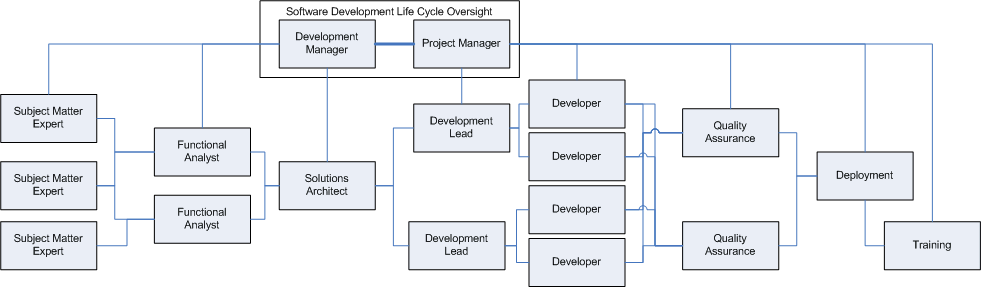
\includegraphics[width=\textwidth]{Fullorgchart1}

\end{frame}

\begin{thebibliography}{99}

\bibitem{Anatomy} \href{https://www.developer.com/tools/article.php/3526491/}{Anatomy of a Software Development Role}
\bibitem{Business} \href{https://itkeys.org/business-analysts/}{Бизнес-аналитики в IT}
\end{thebibliography}

\end{document}
%%% Local Variables: 
%%% mode: TeX-pdf
%%% TeX-master: t
%%% End: 
